\begin{center}
    \begin{tcolorbox}[
        enhanced,
        sharp corners, 
        colback=white,
        boxrule=0pt,
        borderline={0.75pt}{0pt}{black},
        width=\textwidth
        ]
        Interpreting the number and type of solutions to a quadratic equation.
        \tcblower
        \vspace{3.5in}
    \end{tcolorbox}
\end{center}

\begin{myExample}{
    The graph below is for a quadratic function.
    Find the number and type of solutions to the corresponding quadratic equation.
    \begin{center}
        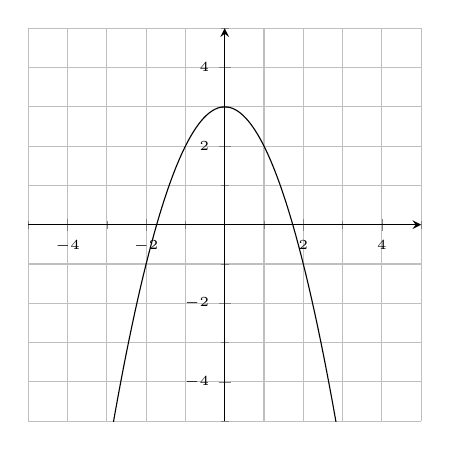
\begin{tikzpicture}
            \begin{axis}[
                width=3in,
                grid=both,
                axis x line = middle,axis y line = middle,
                axis equal image,
                xtick distance = 2, ytick distance = 2, 
                minor tick num = 1,
                xmin = -5, xmax=5,
                ymin = -5, ymax=5,
                tick label style = {font=\tiny},
                ]
                \addplot[no marks, samples=100, domain=-3:4, ] expression { -x^2 + 3 };
            \end{axis}
        \end{tikzpicture}
    \end{center}
}
    \vspace{0.5in}
\end{myExample}

\begin{myExample}{
    The graph below is for a quadratic function.
    Find the number and type of solutions to the corresponding quadratic equation.
    \begin{center}
        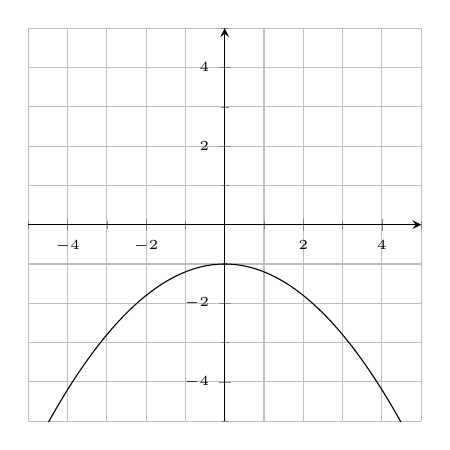
\begin{tikzpicture}
            \begin{axis}[
                width=3in,
                grid=both,
                axis x line = middle,axis y line = middle,
                axis equal image,
                xtick distance = 2, ytick distance = 2, 
                minor tick num = 1,
                xmin = -5, xmax=5,
                ymin = -5, ymax=5,
                tick label style = {font=\tiny},
                ]
                \addplot[no marks, samples=100, domain=-5:5, ] expression { -0.2*x^2 -1 };
            \end{axis}
        \end{tikzpicture}
    \end{center}
}
    \vspace{0.5in}
\end{myExample}
